\documentclass{article}

\usepackage{Styles/header}
\usepackage{Styles/VS2017}

\begin{document}


\begin{titlepage}

    \pagestyle{empty}
    \begin{center}
        \LARGE
            {
                Санкт-Петербургский Государственный Университет \\ Математико-механический факультет
            }
    \end{center}
    \vspace*{45mm}
    
    \begin{center}
        \Large
            {
                Материалы доклада по теме: \\
                {\bf
                    "STL(C++, set, multiset, map, multimap)" \\
                }
            }
    \end{center}
    
    \vspace*{35mm}
    
    \Large
        {
            \noindent
            Выполнил: \hfill студент группы 21.Б12-мм Зернов С. Н. \\
        }
        
    \vspace*{81mm}
    
    \begin{center}
        Санкт-Петербург \\ 2022
    \end{center}

\end{titlepage}

\section{Особенности array и vector}
Выпишем временные оценки работы методов STD::VECTOR:

\begin{center}
    \begin{tabular}{| c || c | c | c | c | c | c | c |}
        \hline
        Контейнер & push\_back & insert & pop\_front & pop\_back & erase & find & count\\ 
        \hline
        std::vector & O(1) & O(n) & O(1) & O(1) & O(n) & O(n) & O(n) \\ 
        \hline
        ? & n/a & O(log n) & n/a & n/a & O(log n) & O(log n) & O(log n) \\
        \hline
    \end{tabular}
\end{center}
Легко заметить, что важнейшие методы работают за линейное время. Задачей данной работы является описание контейнера, позволяющего значительно ускорить операции вставки, удаления и поиска элементов.\\
Во второй строке таблицы отражена временная сложность методов искомого контейнера. \\
\vspace{5mm}

\begin{center}
    \begin{figure}[h]
        \centering
        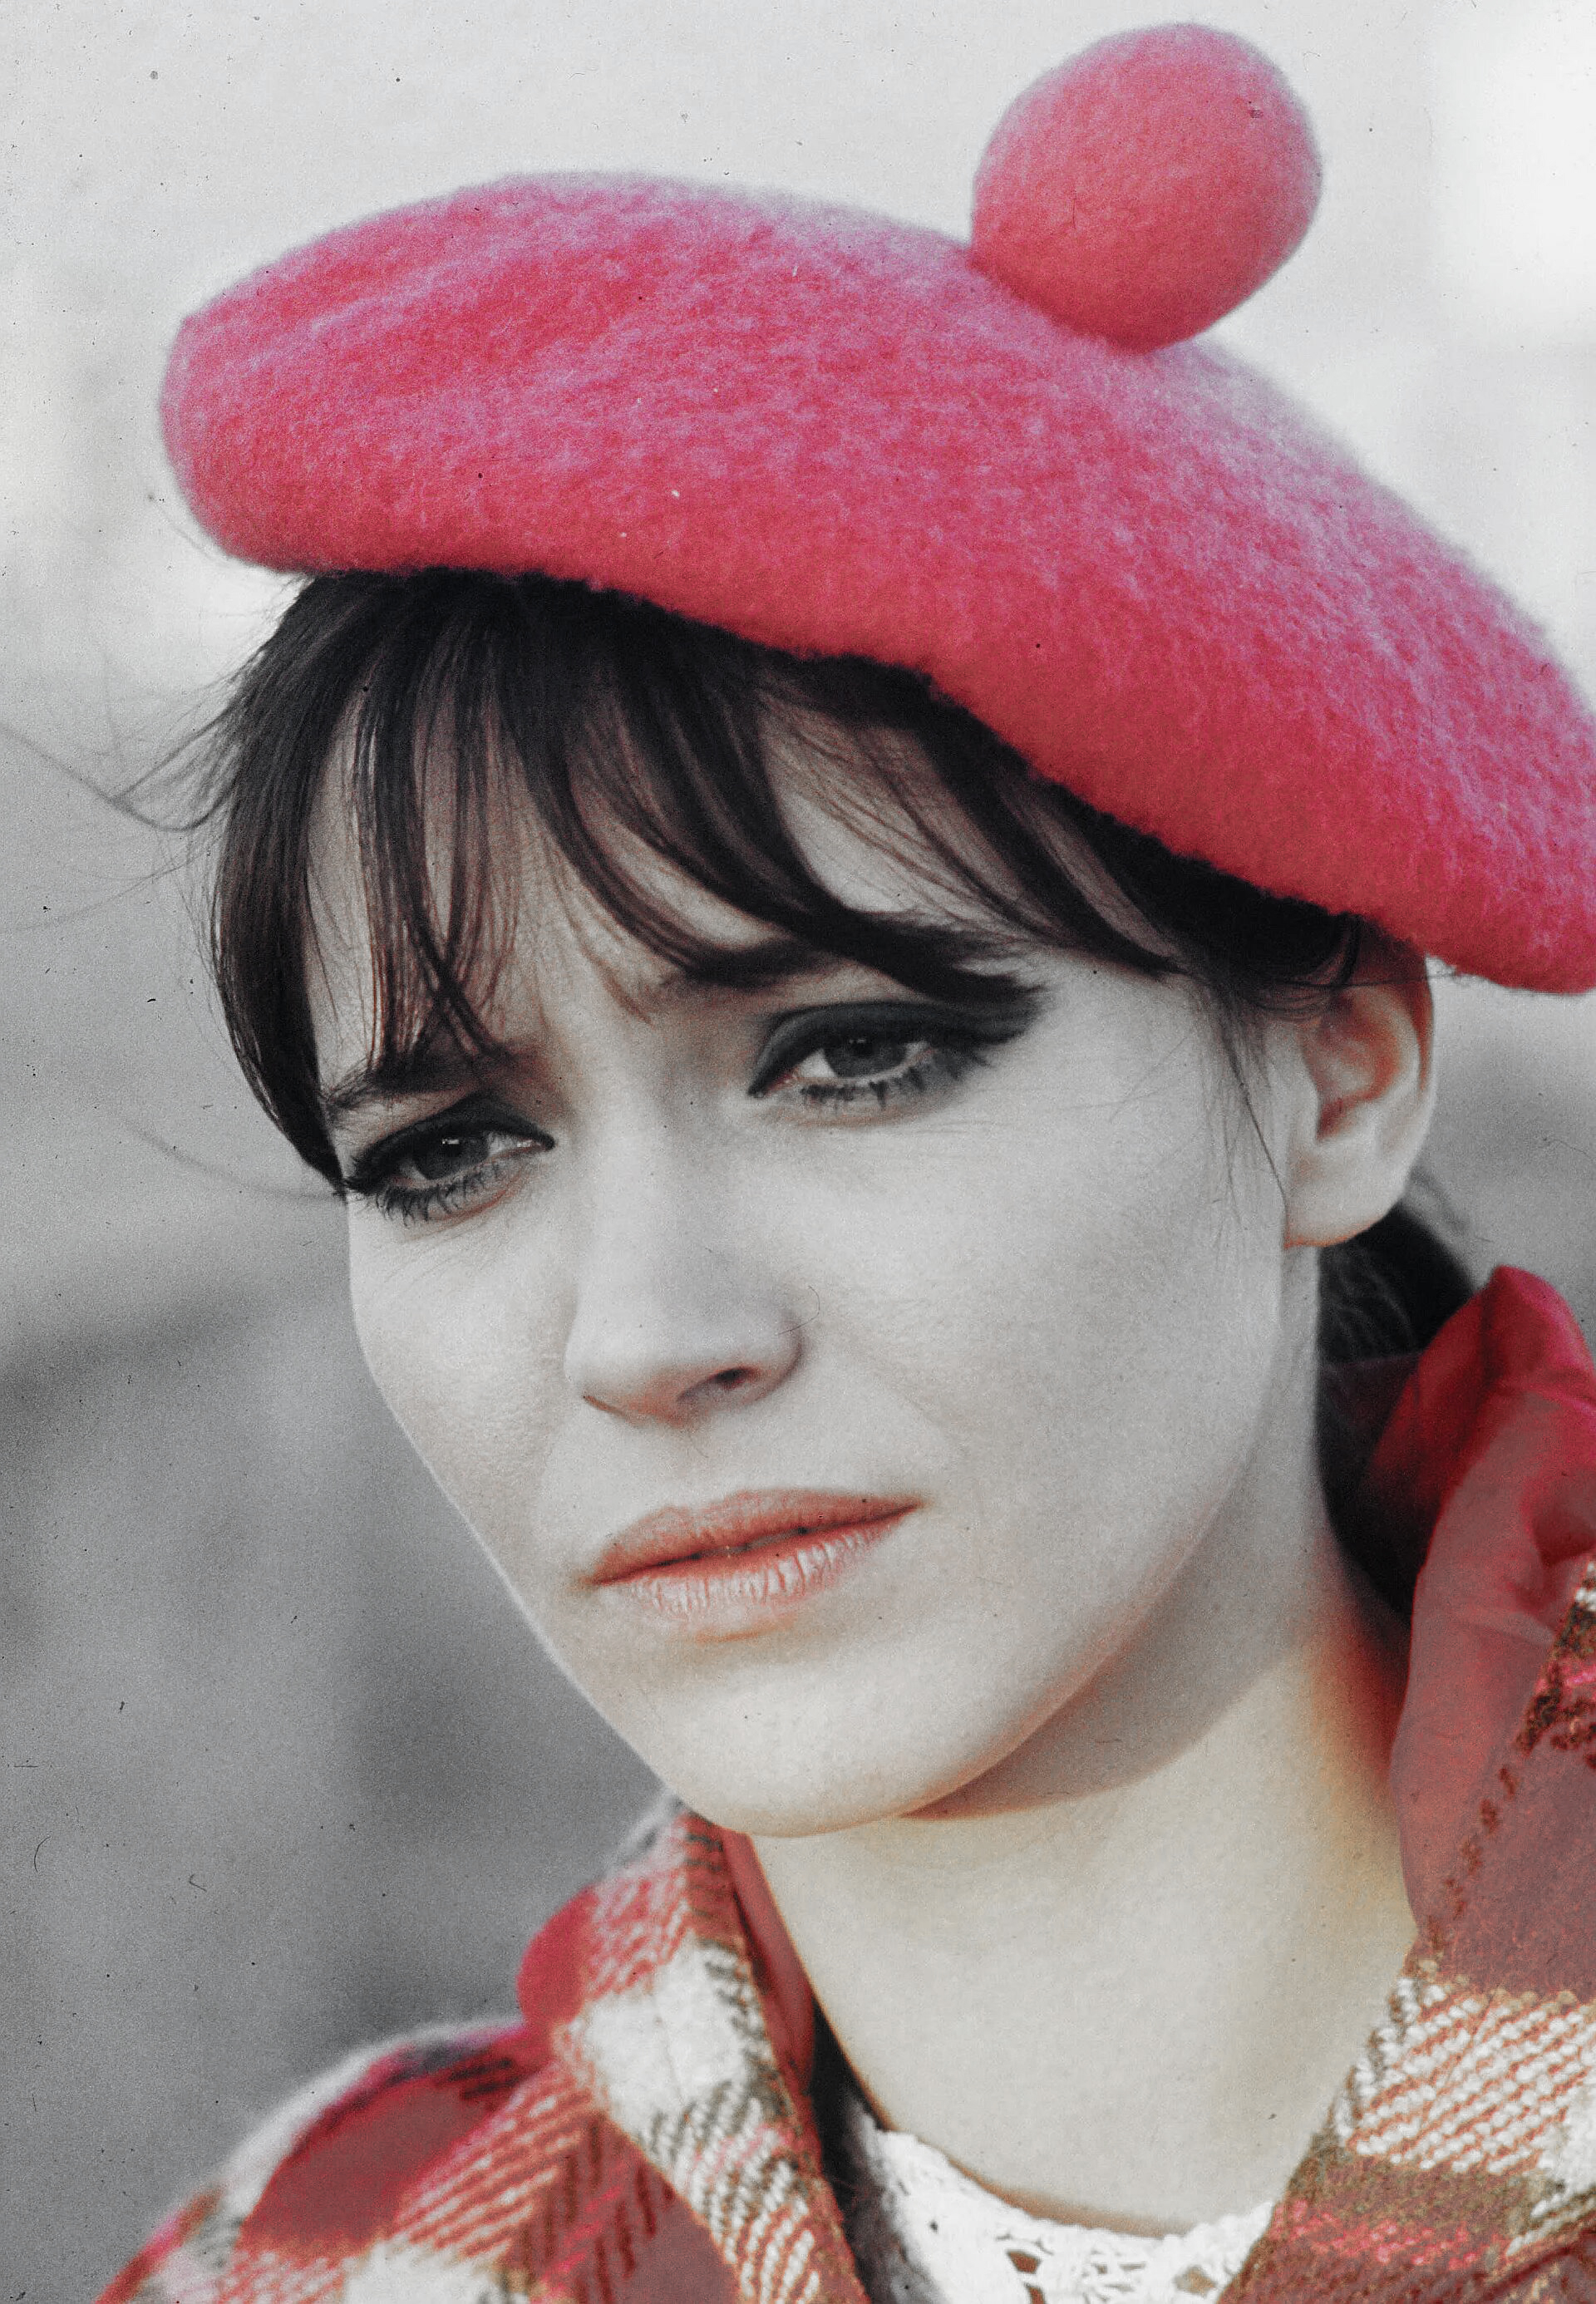
\includegraphics[scale = 0.125]{pictures/annakarinafinal.jpg}
        \caption*{Поиск за O(n) удручает}
    \end{figure}
    \caption{Поиск за O(n) удручает}
\end{center}

\newpage

\section{Красно-чёрные деревья}
Разберёмся с внутренней структурой нашего контейнера. Из-за требуемой логарифмической сложности методов, естественным решением задачи является построение бинарного дерева.\\
Разработчики STL выбрали особый подвид бинарного дерева поиска --- красно-чёрное дерево. Данный параграф будет посвящён его свойствам.\\

\textbf{
    \begin{large}
        Свойства:
    \end{large}
}

\begin{itemize}
    \item Каждый узел окрашен в красный или чёрный цвет
    \item Корень — чёрный \\ 
        \begin{center}
            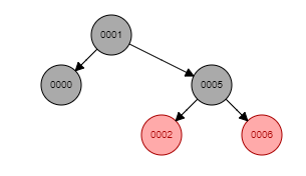
\includegraphics[scale=1]{pic1.png}
        \end{center}
    \item Листья — чёрные NULL-узлы
    \item У каждого красного узла два чёрных потомка \\
        \begin{center}
            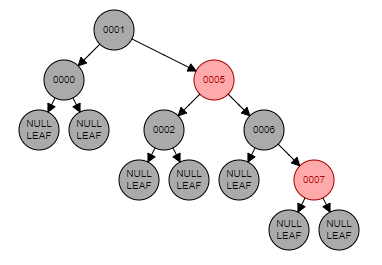
\includegraphics[scale=1]{pic2.png}
        \end{center}
    
    \vspace*{15mm}
    
    \item Пути от узла к его листьям должны содержать одинаковое количество черных узлов \\
        \begin{center}
            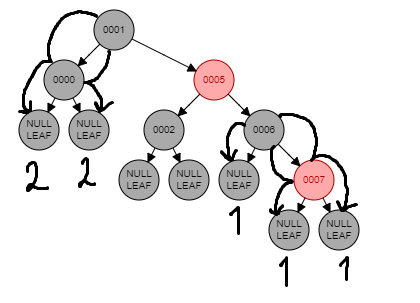
\includegraphics[scale=1]{pic3.png}
        \end{center}
\end{itemize}

\textbf{
    \begin{large}
        Что это даёт?
    \end{large}
}\\
Расположим числа от 1 до 10 в бинарном и красно-чёрном дереве. Представим, что нам надо найти элемент 10: в первом случае на это уйдёт O(n) операций (дерево превратится в связный список), во втором случае мы уложимся в O(log n).\\
\begin{figure}[h]
    \centering
    \begin{subfigure}{0.5\textwidth}
          \centering
          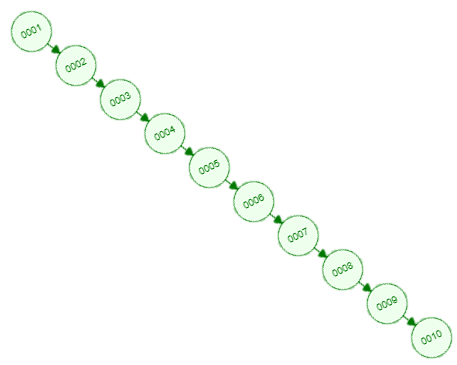
\includegraphics[width=\linewidth]{pic4.png}
          \caption{Бинарное дерево}
          \label{fig:sub1}
    \end{subfigure}%
    \begin{subfigure}{0.5\textwidth}
        \vspace{23mm}
            \centering
                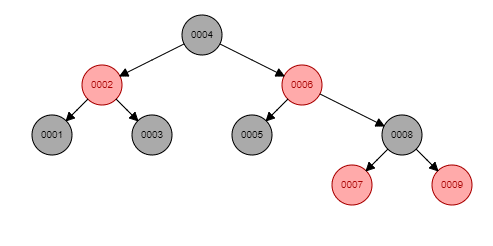
\includegraphics[width=\linewidth]{pic5.png}
                \caption{Красно-чёрное дерево}
                \label{fig:sub2}
            \end{subfigure}
        \label{fig:test}
\end{figure}
Почему разработчики STD выбрали именно красно-чёрное дерево?\\
Ответ:
Операции insert, erase и find выполняются за «железный логарифм»: без вероятностей и усреднений.\\
\vspace{13mm}

Введём дополнительные обозначения: будем называть begin() самый левый узел, а end() — специальный новый узел. Если дерево пустое, то они совпадают.\\
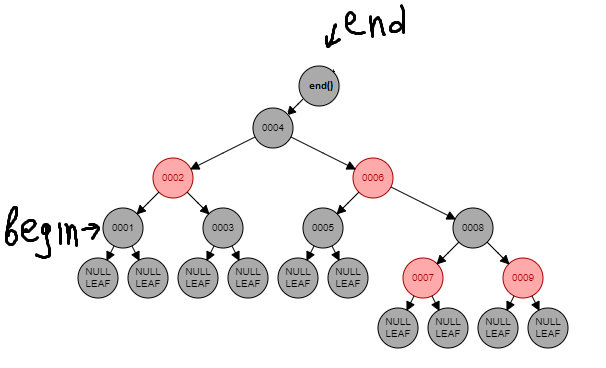
\includegraphics[scale=1]{pic6.png}

Условимся, что у нас есть механизмы вставки (insert) и удаления вершины (erase) из дерева: зачастую они требуют перестройки, а потому непросты в реализации (много случаев)
\begin{figure}[h]
    \centering
    \begin{subfigure}{0.5\textwidth}
          \centering
          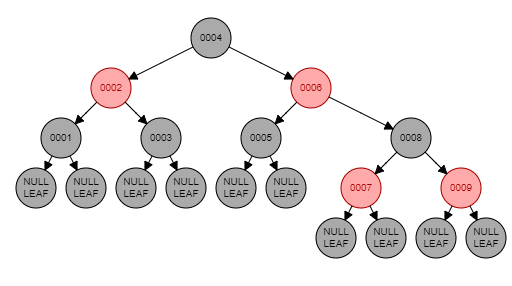
\includegraphics[width=\linewidth]{pic7.png}
          \caption{До удаления вершины с ключём 8}
          \label{fig:sub1}
    \end{subfigure}%
    \begin{subfigure}{0.5\textwidth}
        \vspace{2mm}
            \centering
                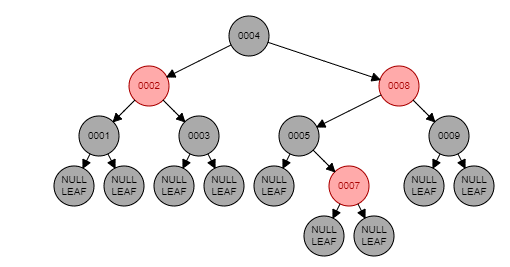
\includegraphics[width=\linewidth]{pic8.png}
                \caption{После}
                \label{fig:sub2}
            \end{subfigure}
        \label{fig:test}
\end{figure}

О \href{https://habr.com/ru/post/557328/}{\underline{вставке}} и \href{https://habr.com/ru/company/otus/blog/521034/}{\underline{удалении}} можно прочитать отдельно.


\newpage


\section{Схематическая реализация std::map}
\begin{center}
    \large{Поля и основные методы}
\end{center}

\lstinputlisting[style=VS2017]{code1.cpp}

\newpage

\textbf{
    \begin{large}
        Опишем полученный класс:
    \end{large}
}

\begin{itemize}
    \item В шаблон передаются типы ключа, значения и компаратор (принцип сравнения ключей). По умолчанию, Compare = std::less<const Key>
    \item Существует четвёртое поле шаблона --- Allocator (для кастомного аллокатора). По умолчанию, Allocator = std::allocator<std::pair<const Key, T>
    \vspace{0mm}
    \item В приватных полях класса хранится внутренняя структура красно-чёрного дерева (цвет вершины и указатели на детей и родителя). Так же указатель на корень и самую левую вершину
    \item в типе Node хранятся пары {const Key, Value}
    \item Итератор возвращает it=std::pair<const Key, Value>
\end{itemize}

\newpage

\section{Методы std::map}
\textbf{
    \begin{large}
        Перечислим основные методы:
    \end{large}
}
\begin{itemize}
    \item operator[] — обращается по ключу к вершине и возвращает ссылку на значение. Если нет такого ключа, то создаёт вершину с ним и присваивает значение по умолчанию
    \item at — похож на operator[], однако не создаёт вершину при отсутсвии ключа
    \item insert — возвращает std::pair<iterator, bool>. Итератор — куда вставилось, bool — произошла ли вставка (если значение с таким ключом есть, то вставка бы не произошла)
    \item erase — по итератору или ключу удаляет вершину дерева
    \item find — по ключу возвращает итератор на вершину
    \item count — считает количество элементов с данным ключом. Для map мало смысла, для multimap актуальна.
\end{itemize}

\section{std::set}

std::set — красно-чёрное дерево, в котором в вершинах хранятся уникальные ключи.
\begin{itemize}
    \item В каком-то смысле std::map без value
    \item Аналог множества в математике
\end{itemize}
\section{Методы std::set}
    Методы аналогичны std::map, однако:
\begin{itemize}
    \item Возвращают уже не std::pair<Key, Value>, а просто Key
    \item Нет оператора []
\end{itemize}

\section{std::multimap и std::multiset}
От стандартных std::map и std::set отличаются лишь тем, что ключи могут повторяться. Поэтому:
\begin{itemize}
    \item Методы доступа к элементам бессмысленны (at, [])
    \item find возвращает по ключу любой из элементов дерева
    \item По существу применимы лишь методы upper\_bound, lower\_bound, equal\_range
\end{itemize}

\section{Методы std::multimap и std::multiset}
\begin{itemize}
    \item upper\_bound — по ключу возвращает первый итератор с не меньшим значением ключа (если его нет, то end())
    \item lower\_bound — по ключу возвращает итератор с не большим значением ключа (аналогично, может вернуть end())
    \item equal\_range — по ключу возвращает промежуток [lower\_bound; upper\_bound)
\end{itemize}
\end{document}
